\section{Introduction}
%This is supplementary material intended for students of introductory Control Theory. It is based off of, and aimed to complement, the course ``Control Theory'' (ERE103) given at Chalmers University of Technology, but is meant to be useful as complementary material for any introductory course on the subject.

This is a supplementary learning material for the course ``Control theory'' (ERE103) at Chalmers University of Technology. The purpose of this material is to give computer science students a more familiar introduction to the subject of control theory. While aimed towards students taking the course ERE103, this learning material is suitable for everyone with an interest in learning more about control theory and is familiar with Haskell. 

The method we use in this material is to create domain-specific languages (DSLs) for the course. A DSL is a programming language specialised for a domain, be it math, physics, astronomy, etc. In our case, we will introduce a new DSL for each section, each specialised for the content of said section. For students who already attended the course ``DSLsofMath'' this approach should be nothing new. For students who have not, additional details are provided throughout the first chapter, ``Prerequisites.''

All DSLs in this material are written in Haskell, so the syntax should be familiar from previous courses. If you are not familiar with Haskell or just want to brush up your skills, we recommend ``Learn you a Haskell for Great Good!'' by Miran Lipovača (\href{http://learnyouahaskell.com/}{http://learnyouahaskell.com/}). 

We hope you find this reading useful. Best of luck!


\todo[inline]{Write about how contact to us in case of errors etc. Write about how the material is not tested.}
\todo[inline]{Maybe add an example of code and an example of pseudocode, ``code will be typeset like this and pseudocode like this''?}

\subsection{Basic control theory}

Control theory studies continuous systems and the control of these. A easy example of a control system, with human input, is when you take a shower. Your body sends signals to the brain when its to hot or cold and you adjust the temperature with your hand. In this case the input is the signal your body sends to your brain and the output is the water temperature. This is a controls system with human input. In control theory we want to automate systems. A example of a common automated control system is the temperature system in your house. A thermostat measures the outside and inside temperature and control the heat elements in you house. This is a control system with two inputs.

\begin{figure}[H]
    \centering
    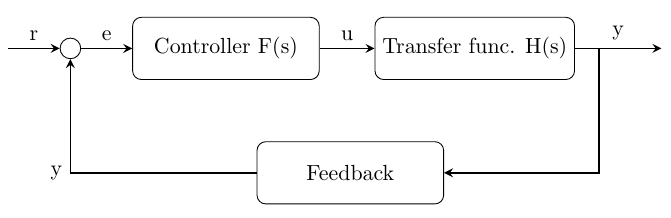
\includegraphics[]{Images/feedback1.PNG}
    \caption{Feedback-loop}
    \label{fig:feed}
\end{figure}


Control systems are created with the combination of measuring a magnitude and a controller. The magnitude measurements and controller create the system input u(t). A system can also utilize the output from the control. This is possible with a feedback loop and is a very common practice in control theory. The quest for all control systems is to create a stable system without delay or overshoot. \todo{(Ska lägga till närmare förklaring för dessa begrepp)} In the course ERE103 this is fulfilled by combining tree different parameters (P, I, D) to create different controllers f(t).  P is just a constant and can decrease the delay of the system. P creates the most basic controller f(t) = P. The I parameter is the integrating part of the controller and is used to remove the stationary fault. The D parameter is used to avoid overshoot. These parameters can be combined to fulfill you specifications.  The most common combination of these parameters in this course are PD, PI and PID. A controller is just a function and can therefore easily be modeled in Haskell.



Control systems are often modelled in block diagrams as you can see above. When we analyze control systems we often transform the functions from the time domain to the frequency domain with the laplace transform. The laplace transform is very useful and will be explained more in-depth later.



In control systems we want our systems to be stable. The results of unstable systems can be horrific so we want to avoid this at all cost. We can use a few methods to ensure this like Ruth-Hurwitz and the Nyqvist Theorem.



